
\subsection{Additional \dataset{} Analysis}

Figure~\ref{fig:object_dist} gives the distributions of target objects $t_o$ across the dialogs in \dataset{}.
The most frequent objects are those that are both frequent across houses and typically number between 2 and 4 per house, and often have a one-to-one correspondence with bedrooms and bathrooms.

\begin{figure}[ht]
\centering
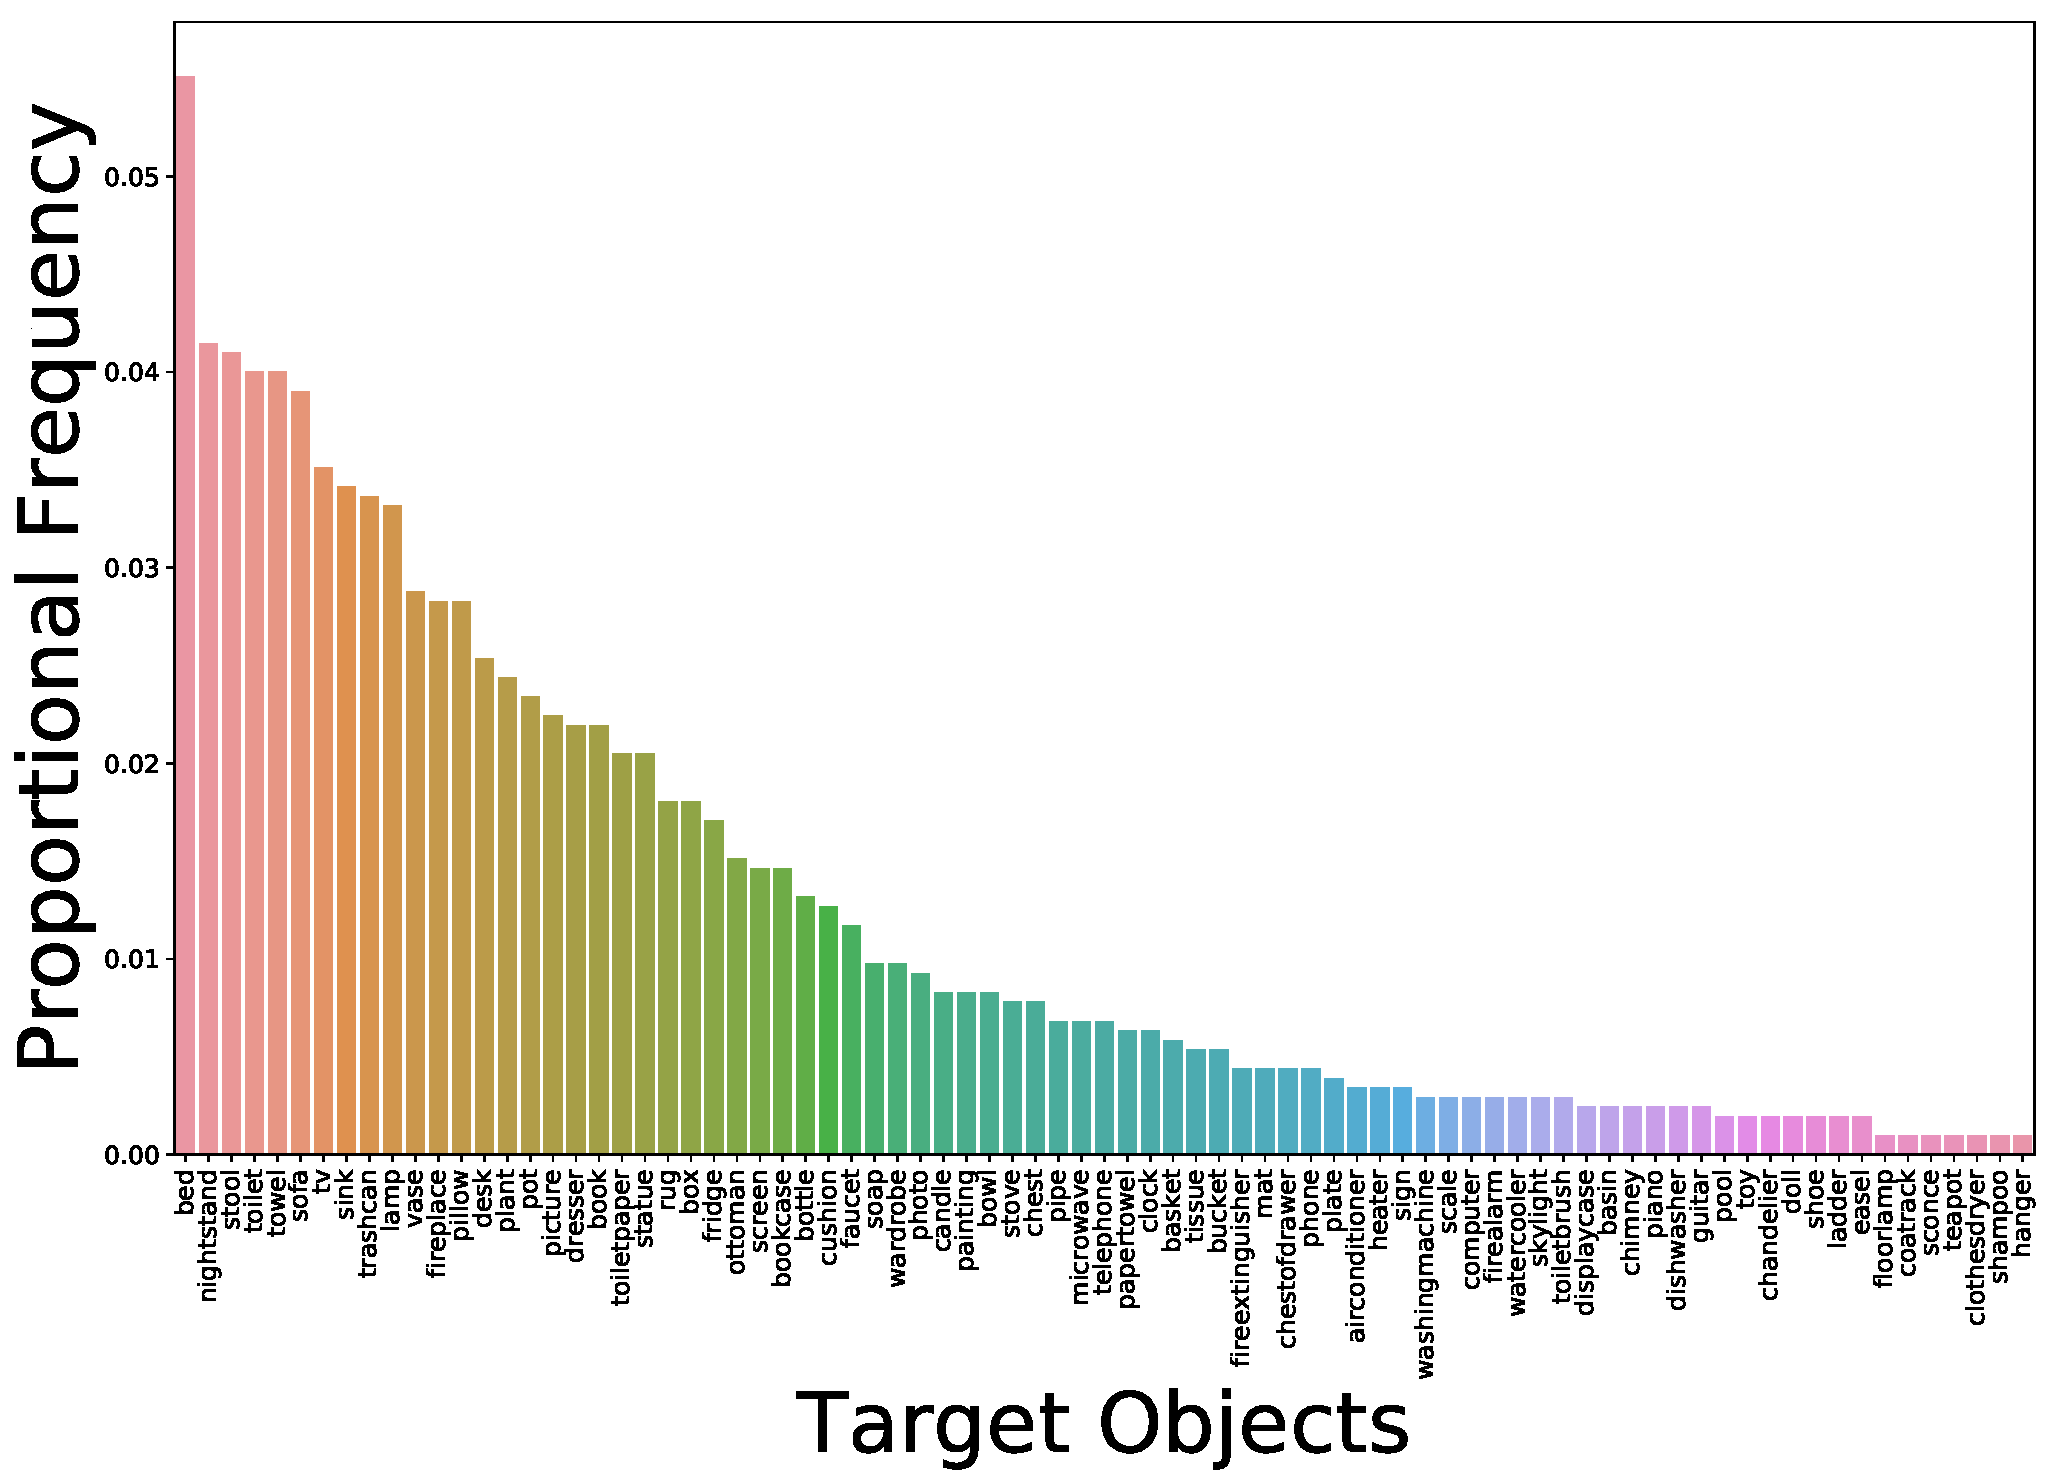
\includegraphics[width=0.9\columnwidth]{figures/target_object_distribution.pdf}
\caption{The distribution of the 81 target objects $t_o$ in dialogs across \dataset{}.}
\label{fig:object_dist}
\end{figure}

Figure~\ref{fig:iou_comp} gives the intersection-over-union (IoU) of paths in \dataset{} within the same scan, comparing them against those in R2R and human performance per-dialog.
The average path IoU across a scan is the average number of navigation nodes in the intersection of two paths over the union of nodes in those paths, across all paths in the scan.
Compared to R2R, the paths in the dialogs of \dataset{} share more navigation nodes per scan because of the way starting panoramas $p_0$ were chosen---to maximize the distance to potential goal regions.
Many \dataset{} paths start at or near the same remote $p_0$ nodes in, e.g., basements, rooftops, and lawns.
Per-dialog, we measure the IoU between human \nav{} and shortest path planner trajectories and find that there is substantially more overlap than between two paths in the same scan, indicating that humans follow closer to the shortest path than to an average walk through the scan (e.g., they are not just memorizing previous dialog trajectories).

\begin{figure}[ht]
\begin{tabular}{cc}
    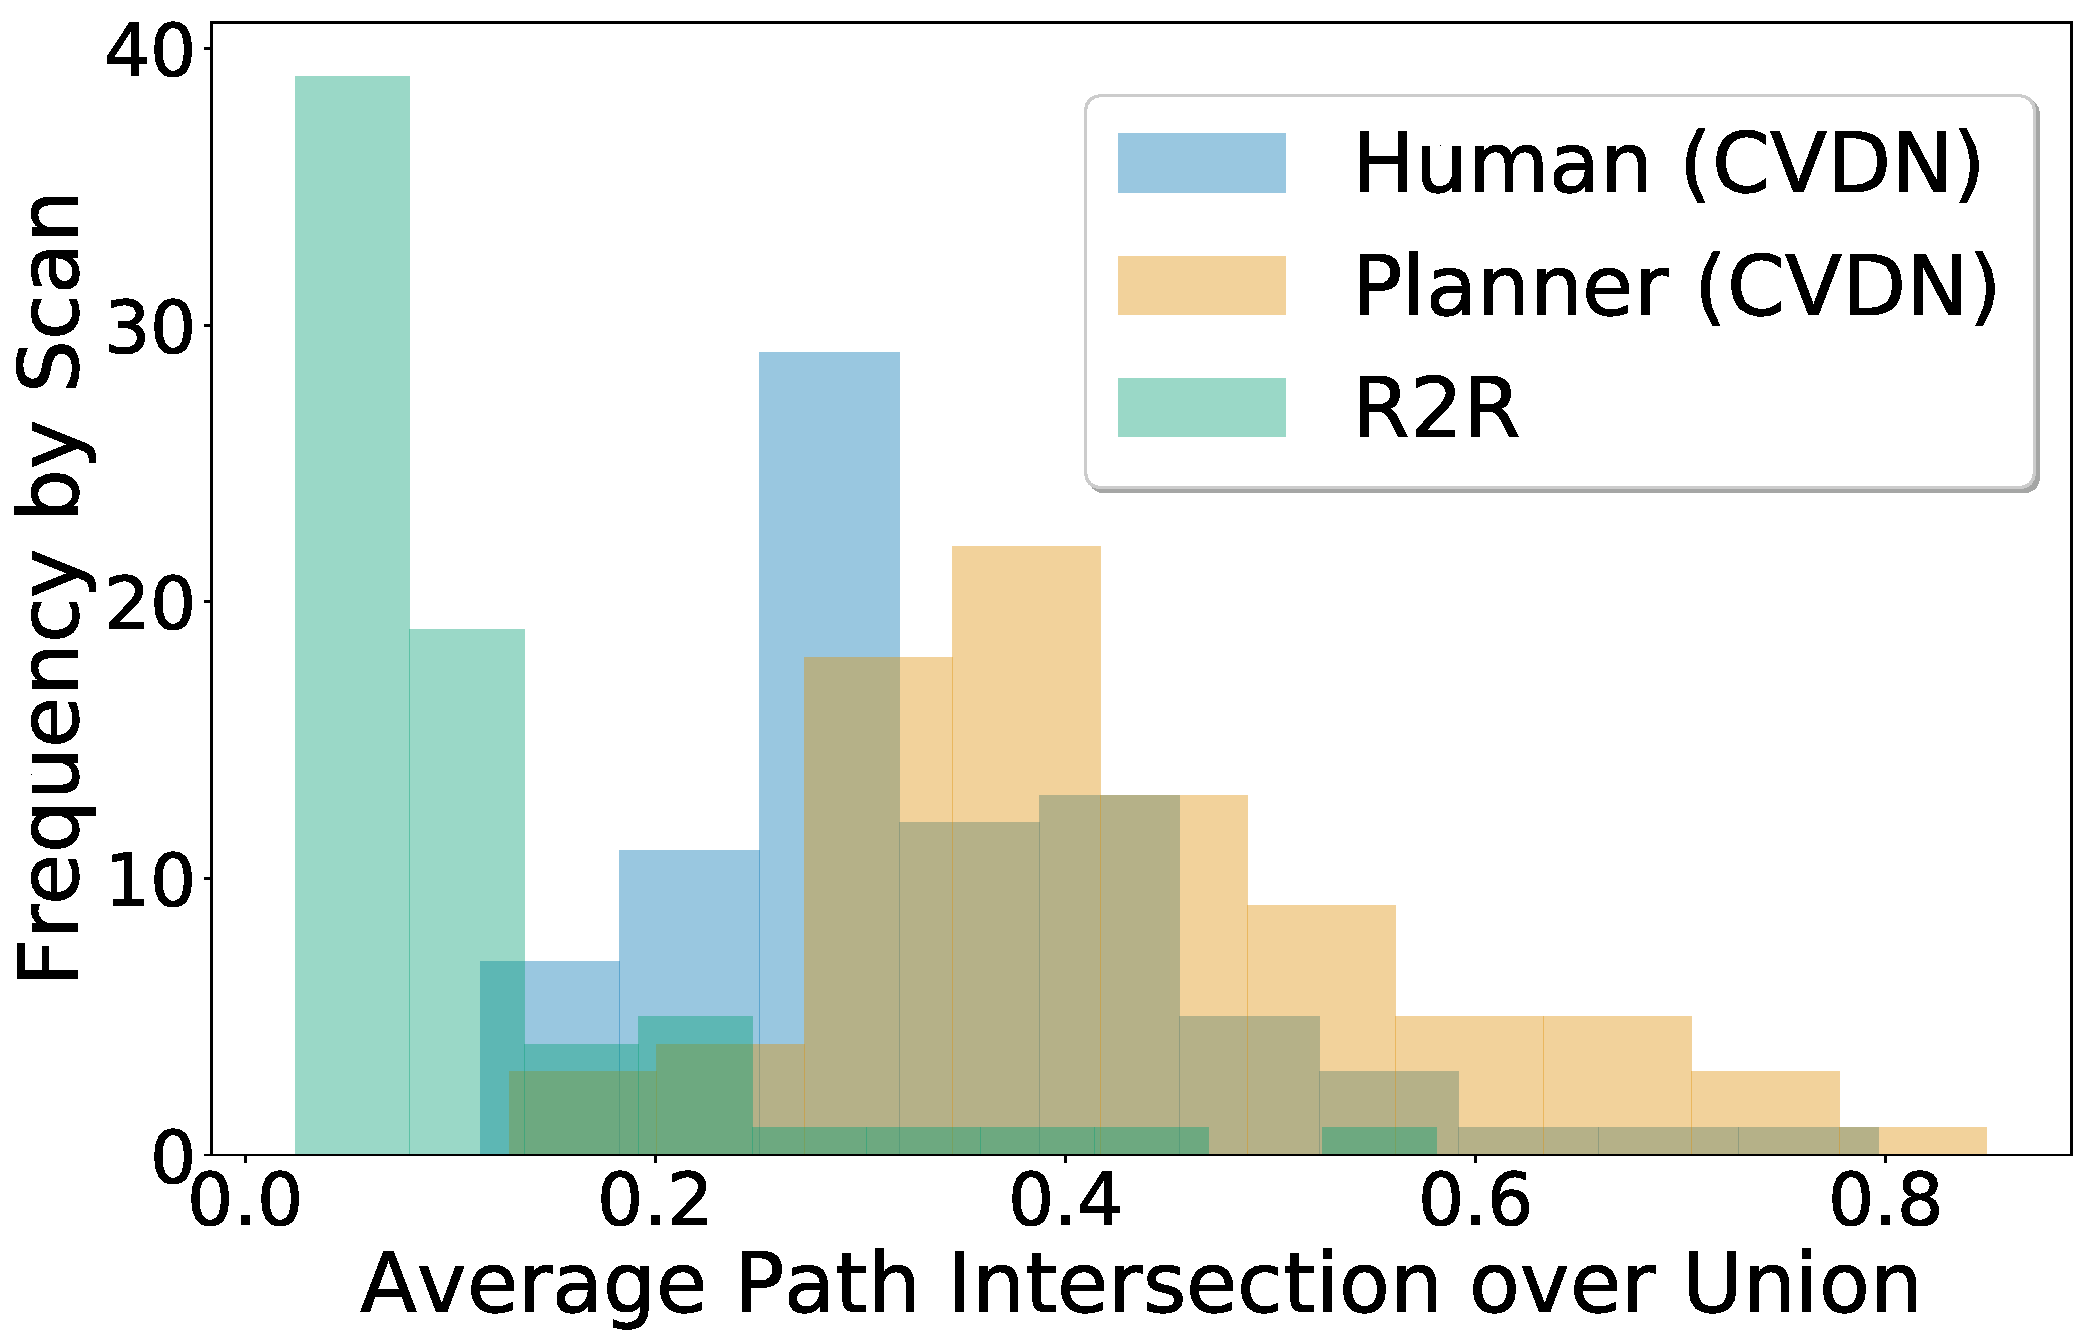
\includegraphics[width=0.45\columnwidth]{figures/iou_mp_comparison.pdf} &
    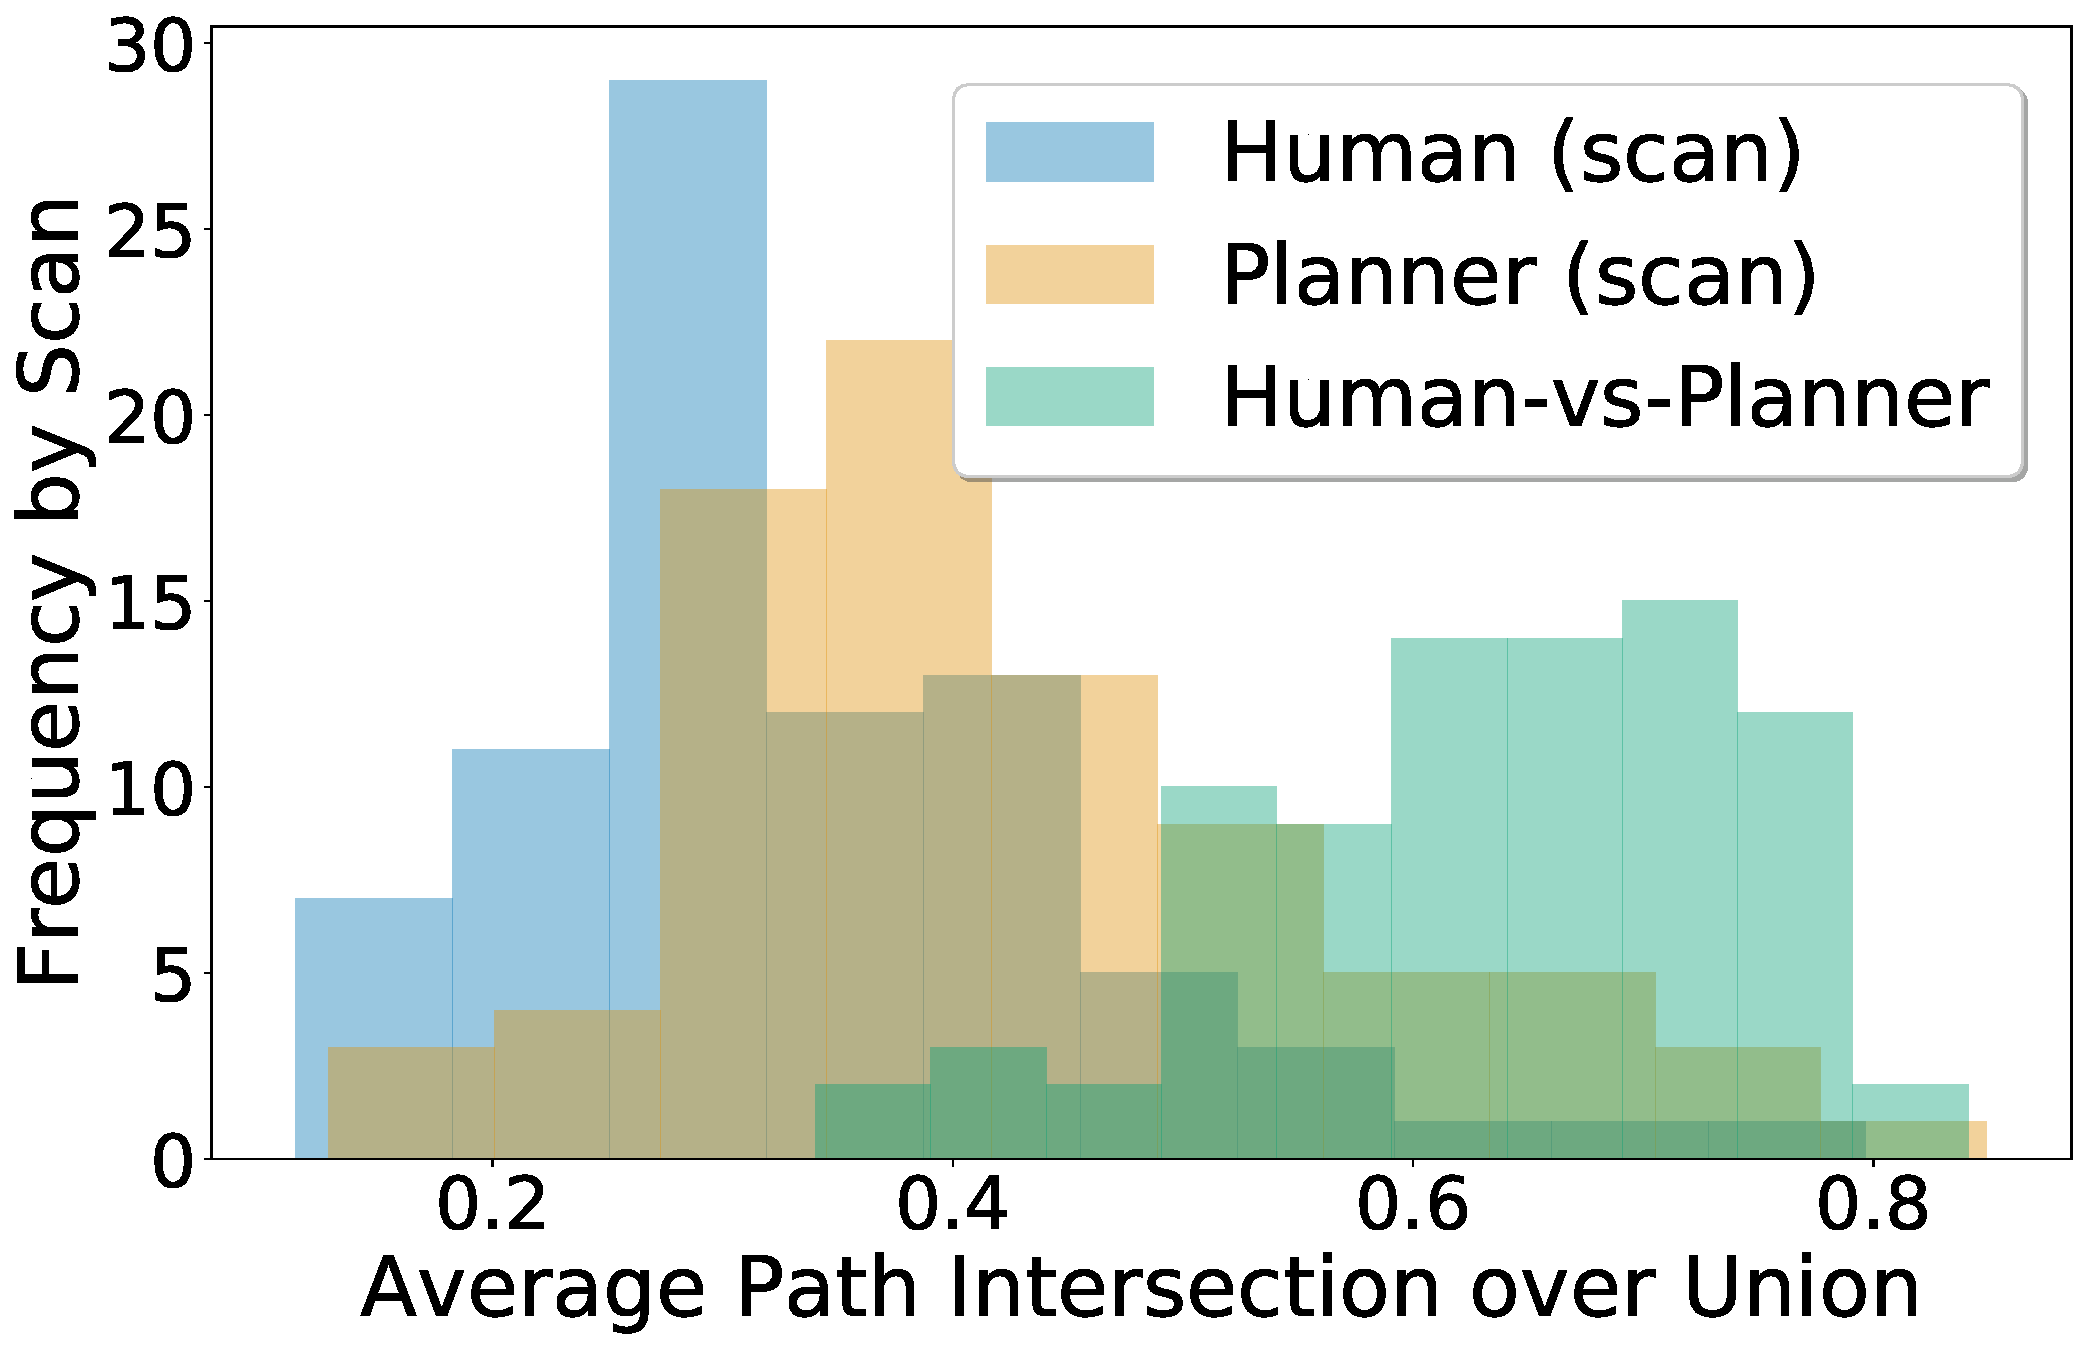
\includegraphics[width=0.45\columnwidth]{figures/iou_human_perf.pdf}
\end{tabular}
\caption{Left: The IoU of nodes in the paths of human \nav{} and shortest path planner trajectories in \dataset{} versus those in R2R when comparing paths in the same scan.
Right: The IoU of \nav{} and shortest path planner trajectories in the same scan versus the IoU of player and shortest path planner trajectories across a dialog.}
\label{fig:iou_comp}
\end{figure}

\subsection{Additional \task{} Analysis}

Figure~\ref{fig:ndh_dists} gives path data for the \task{} task.
Compared to R2R, path lengths using shortest path supervision ($O_i$) are on average shorter than those in R2R, because paths shown to the \ora{} were at most length 5.
By contrast, human \nav{} paths ($N_i$) are substantially longer than those seen in R2R.
We also examine the distribution of the number of hops progressed towards the goal per \task{} instance across \ora{} shortest path, human navigator, and mixed supervision ($M_i$).
While the planner always moves towards the goal (or stands still, if the \nav{} is already in the goal region), human \nav{}s sometimes move farther away from the goal, though in general make more progress than the planner.
Using mixed supervision, fewer trajectories move ``backwards''; the simple heuristic of whether a \nav{} walked over the last node in the \ora{}'s described shortest path shifts the distribution weight farther towards positive goal progress.

\begin{figure}[ht]
\begin{tabular}{cc}
    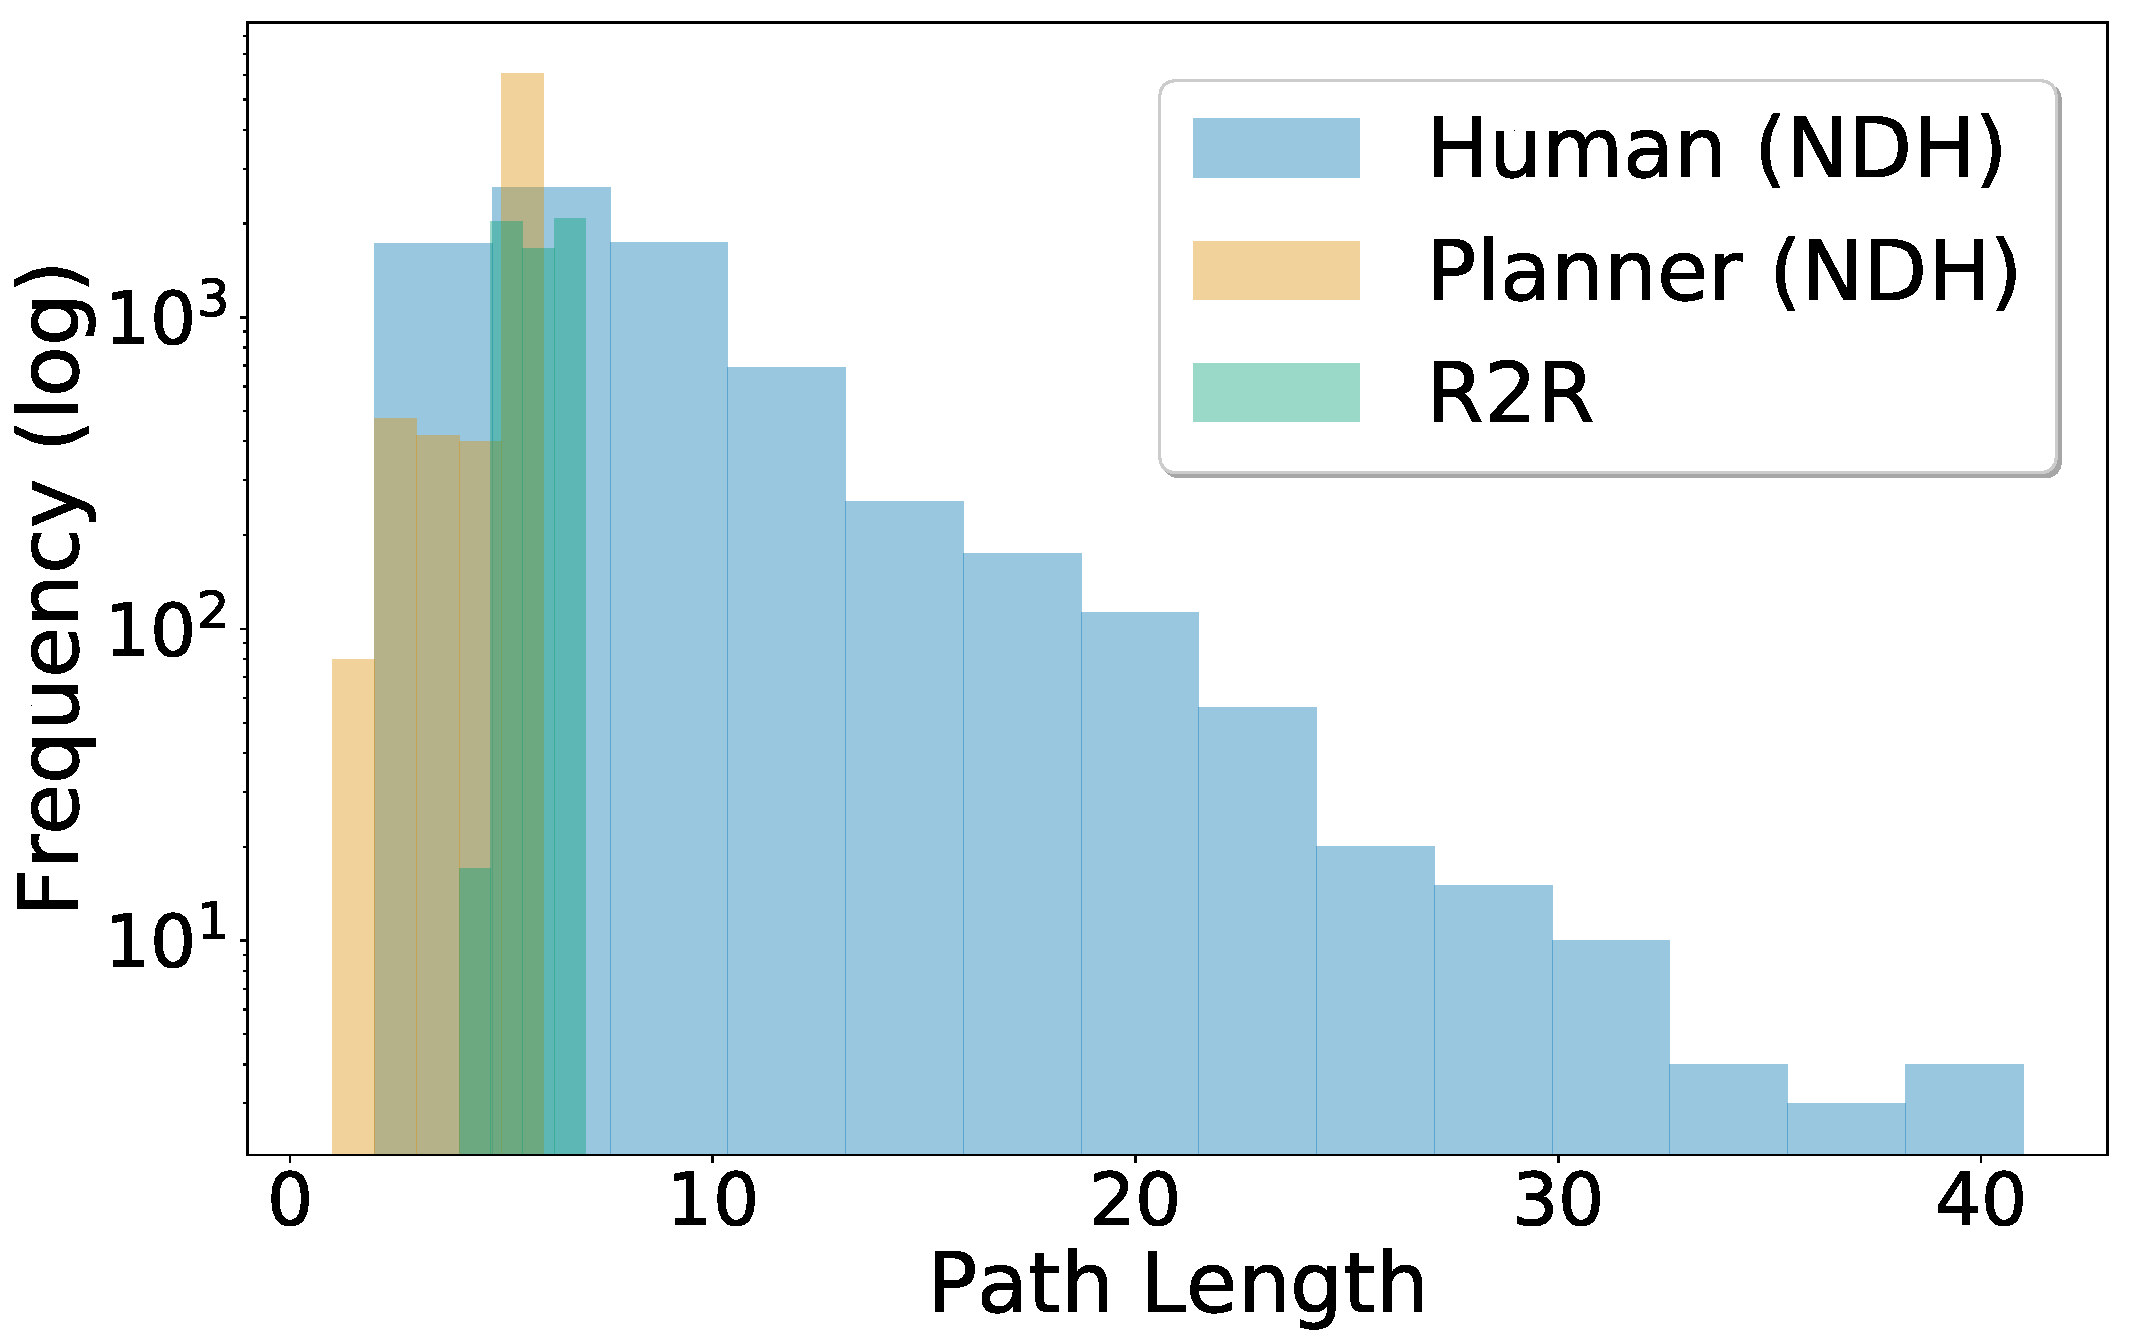
\includegraphics[width=0.45\columnwidth]{figures/path_len_per_ndh.pdf} &
    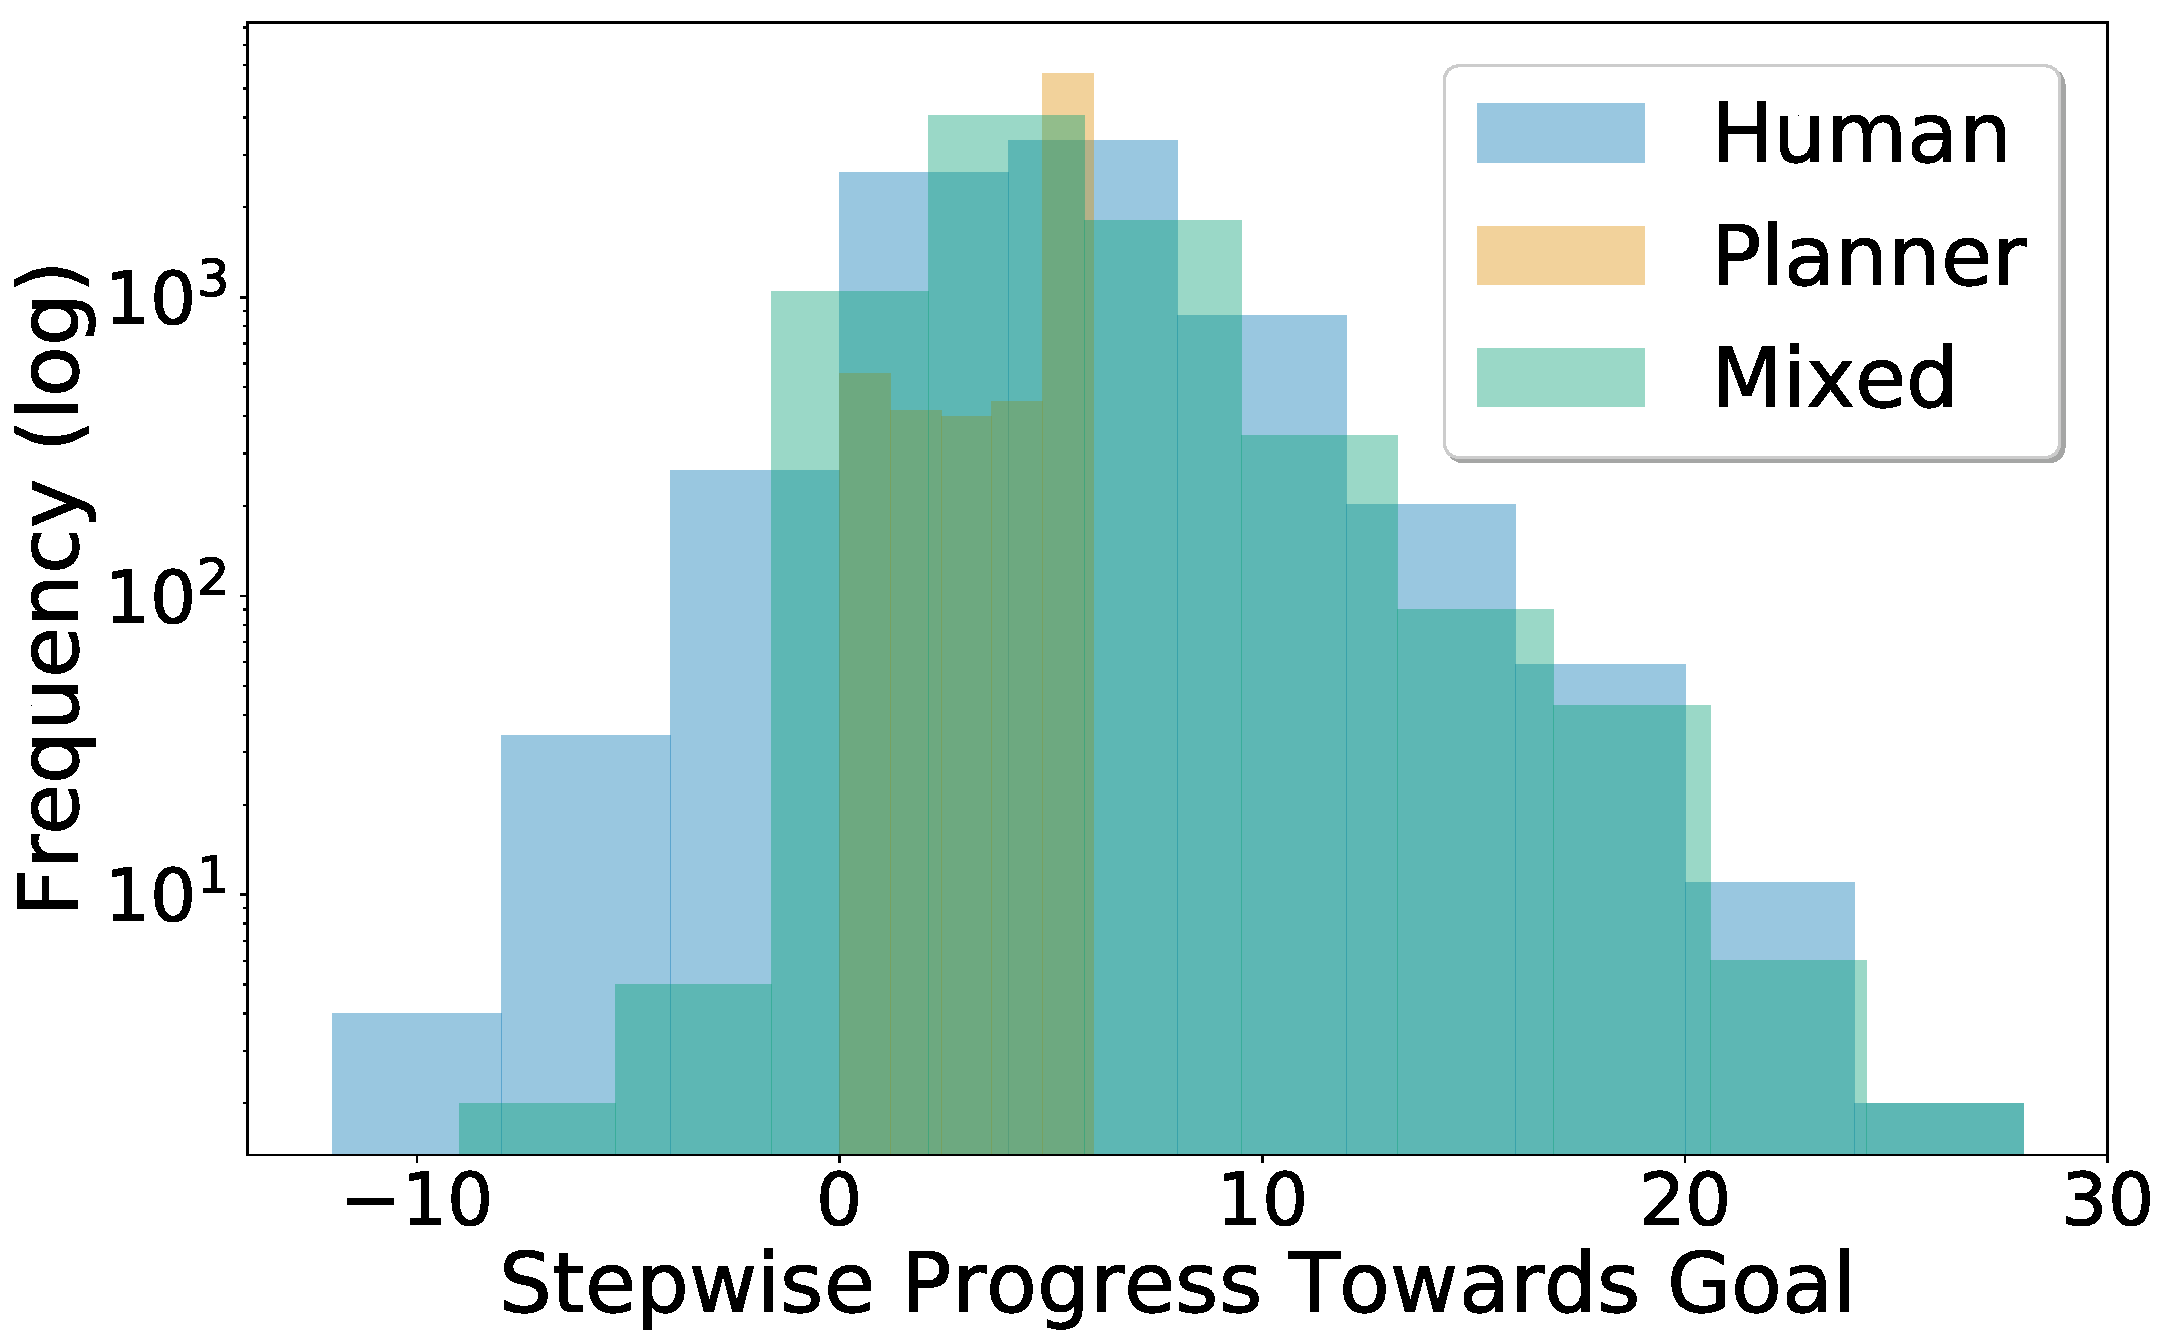
\includegraphics[width=0.45\columnwidth]{figures/goal_red_per_ndh.pdf}
\end{tabular}
\caption{Left: The distributions of path lengths by human \nav{} and the shortest path planner provided as supervision in \task{} instances versus path lengths in R2R supervision.
Right: The progress per NDH instance made towards the goal (in steps) by the human \nav{}, the shortest path planner, and the mixed-supervision path.}
\label{fig:ndh_dists}
\end{figure}

\subsection{\task{} Model Performance Statistical Comparisons}
We ran paired $t$-tests between all model ablations within each supervision paradigm (e.g., comparing all mixed supervision models to one another), and across paradigms (e.g., comparing the full dialog history model trained with mixed supervision to the one with navigator path supervision).
Data pairs are NDH the distances progressed towards the goal on the same instance (i.e., dialog history and goal) between two conditions.
This results in hundreds of comparison tests, so we apply a Benjamini--Yekutieli procedure to control the false discovery rate.
Because the tests are not all independent, but some are, we estimate $c(m)$ under an arbitrary dependence assumption as $c(m)~=~\sum_{i+1}^{m}{\frac{1}{i}}$, where $m$ is the number of tests run.
We choose a significance threshold of $\alpha<0.05$.
Rather than report the hundreds of individual $p$-values, we highlight salient results below.

\paragraph{Different forms of supervision}
With one exception, in all environments (\emph{seen} validation, \emph{unseen} validation, and \emph{unseen} test), across ablations of language context (i.e., full model using all history down to model using only the target object as dialog context), the differences in progress towards the goal under oracle, navigator, and mixed supervision are statistically significantly different.
The only exception is the difference between oracle and navigator path supervision in \emph{unseen} validation environments with the last answer only (i.e., row 16 of Table~\ref{tab:navigation}) ($p=0.006$).
Models trained with mixed supervision almost always achieve the most progress. For brevity, below we discuss further comparisons between models trained with mixed supervision.

\paragraph{Different amounts of dialog history}
In \emph{unseen} validation and test environments, using all dialog history statistically significantly outperforms using only the target object, but not only the last answer ($p=0.773$ in validation, $p=0.035$ in test) or the last question-answer exchange ($p=0.143$ in validation, $p=0.560$ in test).
Notably, in test environments, a statistically significant difference compared to using only the target object is observed \emph{only} when using all dialog history.
In \emph{seen} validation houses, adding additional dialog history does not result in statistically significant gains, reflecting the representative power of the vision-only unimodal baseline.

\paragraph{Unimodal ablations}
In \emph{unseen} validation and test environments, the model using all dialog history statistically significantly outperforms the unimodal baselines in all cases except the language-only unimodal model in the \emph{unseen} validation houses ($p=0.011$).
In \emph{seen} validation houses, this model statistically significantly outperforms the language-only and zero (no language, no vision) unimodal ablations.
This result does not hold for the vision-only baseline, which is able to memorize the familiar houses for use at test time.


\subsection{Sequence-to-Sequence Model Training}

\paragraph{Hyperparameters.}
We use the training hyperparameters (optimizer, learning rate, hidden state sizes, etc.) presented in \citet{anderson:cvpr18} when training our sequence-to-sequence agents.
We adjust the maximum input sequence length for language encoding based on the amount of dialog history available: 3 for $t_o$ only (e.g., \texttt{TAR} tag, the target itself, and \texttt{EOS}); 70 for $A_i$; 120 for adding $Q_i$; and 720 (e.g., 120 times 6 turns of history) for $Q_{1:k},A_{1:k}$.
We increase the maximum episode length (e.g., the maximum number of navigation actions) depending on the supervision being used: 20 for oracle $O_i$ (the same as in R2R) and 60 for navigator $N_i$ and mixed $M_i$.

\paragraph{Teacher- versus Student-Forcing.}
We use student-forcing when training all of our sequence-to-sequence agents.
\citet{anderson:cvpr18} found that student-forcing improved agent performance in unseen environments.
Further, \citet{thomason:naacl19} found that agents trained via teacher-forcing were outperformed by their unimodal ablations (i.e., they did not learn to incorporate both language and vision supervision, instead memorizing unimodal priors).
Thus, we see no value in evaluating multi-modal agents trained via teacher-forcing in this setting.

\paragraph{Language Encoding.}
It is common in sequence-to-sequence architectures to reverse the input sequence of tokens during training, because the tokens relevant for the first decoding actions are likely also the first in the input sequence.
Reversing the sequence means those relevant tokens have been seen more recently by the encoder, and this strategy was employed in prior work~\cite{anderson:cvpr18}.
Following this intuition, we preserve the order of the dialog history during encoding, so that the most recent utterances are read just before decoding, but reverse the tokens at the utterance level (e.g., $Q_i$ in Figure~\ref{fig:model} is represented as sequence ``\texttt{<NAV>} ? upstairs go I Should'').

\subsection{Naive Dialog History Encoding}

We naively concatenated an encoded navigation history $N_H$ (via an LSTM taking in ResNet embeddings of past navigation frames) to the encoded dialog history, then learned a feed-forward shrinking layer to initialize the decoder (Table~\ref{tab:navigation_history_appendix}).
We hypothesize that there is some signal in this information, but we discover that naive concatenation does not improve performance in \textit{seen} or \textit{unseen} environments.
We suspect that a modeling approach which learns an attention alignment between the navigation history and dialog history could make better use of the additional signal.

\begin{table}[ht]
\centering
\begin{small}
\begin{tabular}{ccccccc>{\raggedleft\arraybackslash}p{1.5cm}>{\raggedleft\arraybackslash}p{1.5cm}>{\raggedleft\arraybackslash}p{1.5cm}}
    & \multicolumn{6}{c}{\textbf{Seq-2-Seq Inputs}} & \multicolumn{3}{c}{\textbf{Goal Progress} (m) $\uparrow$} \\
    & & & & & & $Q_{1:i-1} $ & & & \\
    \textbf{Fold} & $N_H$ & $V$ & $t_o$ & $A_i$ & $Q_i$ & $A_{1:i-1}$ & \textbf{Oracle} & \textbf{Navigator} & \textbf{Mixed} \\
    \toprule
    \multirow{3}{*}{\rotatebox[origin=c]{90}{Val (Se)}} & \multicolumn{6}{c}{\texttt{Shortest Path} Agent} & $8.29$ & $7.63$ & $9.52$ \\
    & & \cblkmark & \cblkmark & \cblkmark & \cblkmark & \cblkmark & $4.48$ & $5.67$ & $5.92$ \\
    & \cblkmark & \cblkmark & \cblkmark & \cblkmark & \cblkmark & \cblkmark & $4.47$ & $5.37$ & $5.82$ \\
    \midrule
    \multirow{3}{*}{\rotatebox[origin=c]{90}{Val (Un)}} & \multicolumn{6}{c}{\texttt{Shortest Path} Agent} & $8.36$ & $7.99$ & $9.58$ \\
    & & \cblkmark & \cblkmark & \cblkmark & \cblkmark & \cblkmark & $1.23$ & $1.98$ & $2.10$ \\
    & \cblkmark & \cblkmark & \cblkmark & \cblkmark & \cblkmark & \cblkmark & $1.19$ & $1.86$ & $1.84$ \\
    \bottomrule
\end{tabular}
\end{small}
\caption{
Average sequence-to-sequence agent performance when the agent encodes the entire navigation history $N_H$ compared against the \texttt{Shortest Path} upper bound and the agent encoding all dialog history across different supervision signals.
}
\label{tab:navigation_history_appendix}
\end{table}
